\begin{frame}\frametitle{Задачи}
    \begin{itemize}
        \item Обеспечить загрузку входных данных
        \item Визуализировать результаты поиска объекта
        \item Склеить написанный код в единый проект
    \end{itemize}
\end{frame}

\begin{frame}\frametitle{Процесс разработки}
    Написаны:
    \begin{itemize}
        \item модуль для загрузки ключевых кадров
        \item интерфейс командной строки для работы с ними
        \item рендер объекта при помощи OpenGL
        \item пользовательский интерфейс для удобства работы
    \end{itemize}
\end{frame}

\begin{frame}\frametitle{Загрузка ключевых кадров}
    \begin{itemize}
        \item Сканирует директорию и ищет в ней объект и ключевые кадры в 
            заданном формате
        \item Считывает их
        \item Выдает класс, содержащий информацию о ключевом кадре --- KeyFrame
    \end{itemize}
    Структура KeyFrame
    \begin{itemize}
        \item Положение и поворот камеры
        \item Внутренние параметры камеры
        \item Положение и поворот объекта
    \end{itemize}
\end{frame}

\begin{frame}\frametitle{GUI. Структура}
    \begin{itemize}
        \item Панель инструментов с кнопками для запуска алгоритмов поиска 
            объекта
        \item Виджет с вкладками, содержащими ключевые кадры
    \end{itemize}
    Структура вкладки:
    \begin{itemize}
        \item Картинка
        \item Модель, отрисованная поверх нее в виде сетки
    \end{itemize}
\end{frame}

\begin{frame}\frametitle{Технологии}
    \begin{itemize}
        \item PySide (Qt) - GUI
        \item OpenGL      - Отрисовка модели объекта на ключевом кадре
    \end{itemize}
\end{frame}

\begin{frame}\frametitle{GUI}
    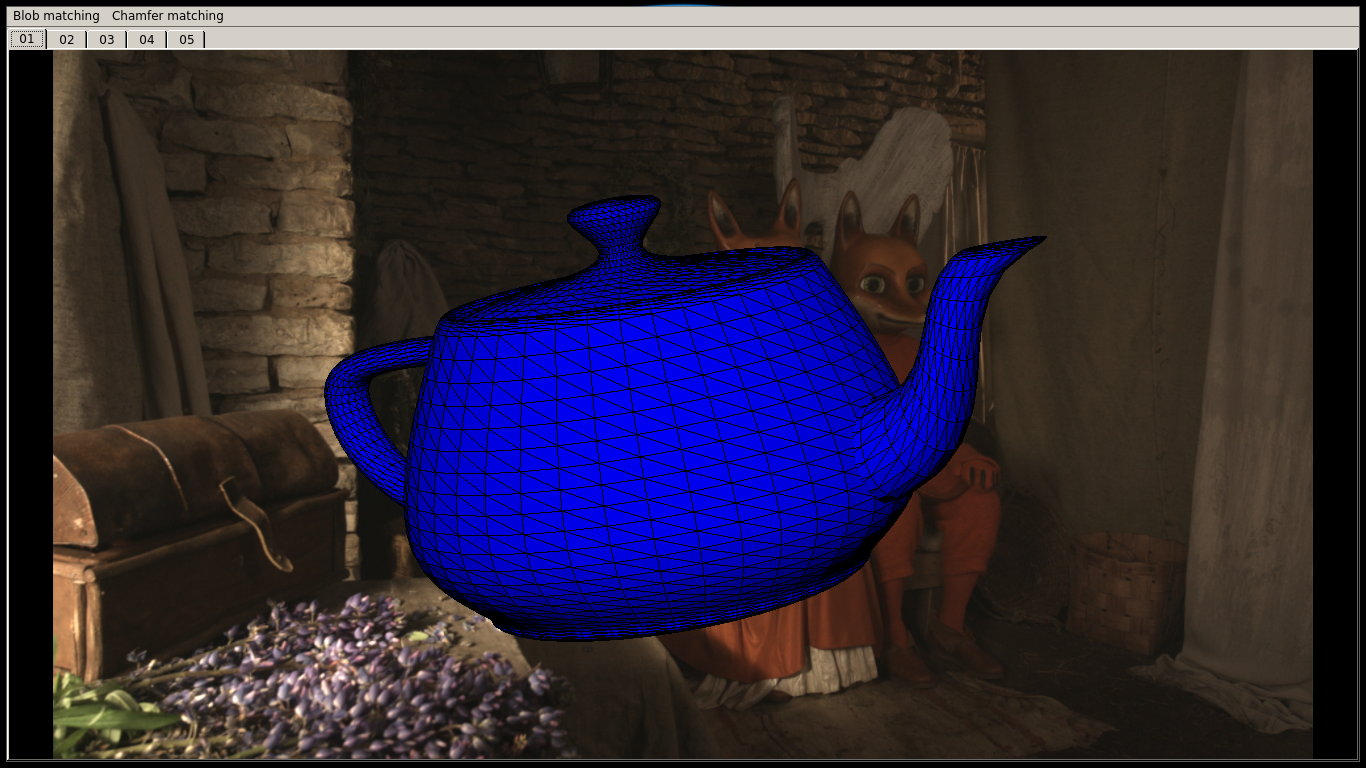
\includegraphics[height=6cm]{gui_samples/sample_01.png}
\end{frame}

\begin{frame}\frametitle{GUI}
    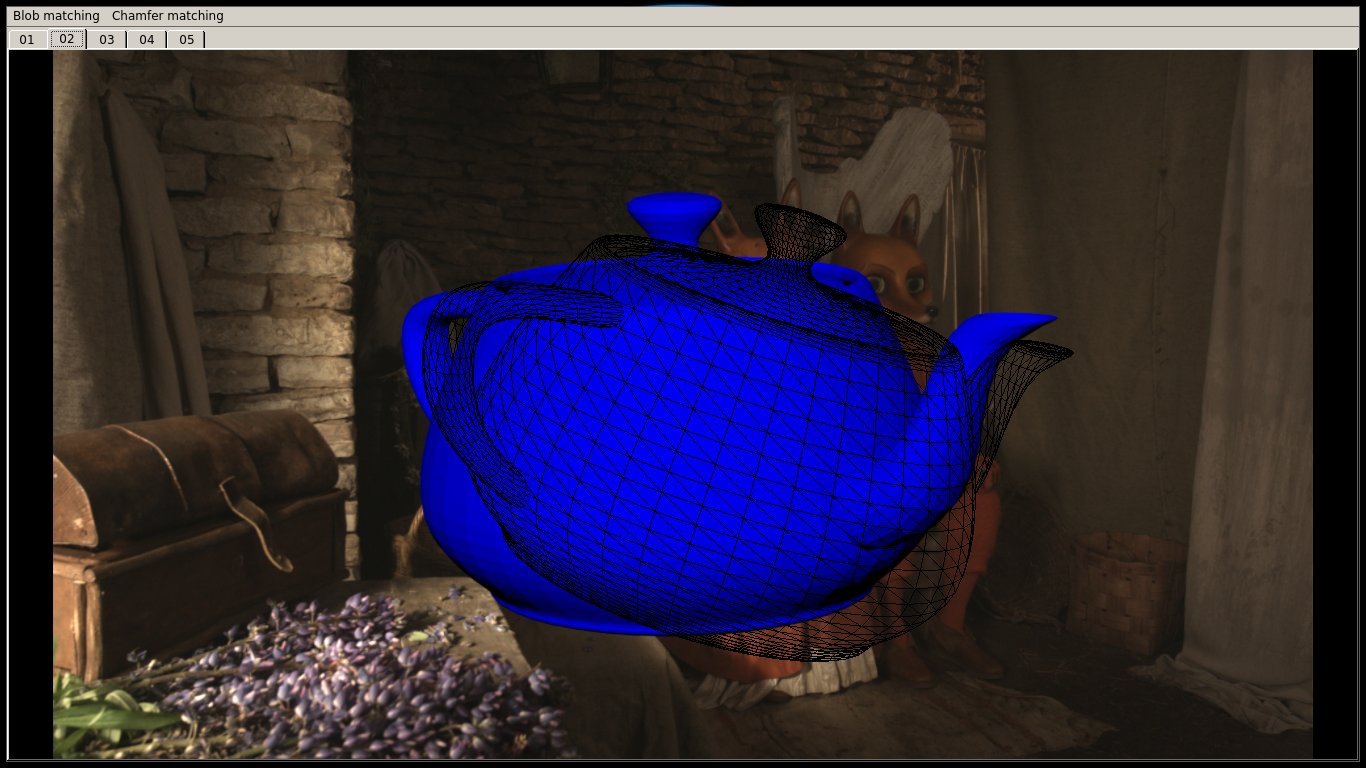
\includegraphics[height=6cm]{gui_samples/sample_02.png}
\end{frame}

\begin{frame}\frametitle{Склейка кода}
    Структура проекта
    \begin{itemize}
        \item main
        \item loading
        \item matching
            \begin{itemize}
                \item chamfer
                \item blob
            \end{itemize}
        \item gui
            \begin{itemize}
                \item main window
                \item key frame previewer
            \end{itemize}
    \end{itemize}
\end{frame}

\begin{frame}\frametitle{Результаты}
    \begin{itemize}
        \item Получился относительно цельный проект
        \item Все работает и шуршит
        \item Я разобрался с OpenGL и его использованием в Qt
        \item Получил опыт разработки в команде и работы с Github
    \end{itemize}
\end{frame}
